\documentclass[english,oneside,color]{htldipl}
% Zulässige Class Options:
%   Hauptsprache: german (default), english
%   Doppelseitig: oneside (default), twoside
%   Syntax-Highlighting: color (default), black

% die folgende Zeile einkommentieren für Arial-Ähnliche Schriftart
%\renewcommand{\familydefault}{\sfdefault}

\graphicspath{{images/}}    % wo liegen die Bilder?

\usepackage{geometry}
\usepackage{hyperref}
\usepackage{float}

\geometry{
	a4paper,
	margin=3cm,
	top=1.5cm
}

%%%----------------------------------------------------------
\begin{document}
%%%----------------------------------------------------------

\title{GRAMOC - Gradienten Magnetometer Online Controller}

\abteilung{Informatik}
\schwerpunkt{}
\studienort{Wiener Neustadt}
\schule{HTBLuVA Wiener Neustadt}
\schullogo{htl.jpeg}
\abgabejahr{2017/18}

\betreuerA{Dr. Michael Stifter}
\betreuerB{}
\betreuerC{}
%\betreuerD{} leer lassen wenn nicht vorhanden

\schuelerA{Nico Kratky}
\evidenzA{5CHIF-13}
\subthemaA{Entwicklung Server, Netzwerkprotokoll}

\schuelerB{Nico Leidenfrost}
\evidenzB{5CHIF-14}
\subthemaB{Entwicklung App, Visualisierung}

\schuelerC{}
\evidenzC{}
\subthemaC{}

\schuelerD{}
\evidenzD{}
\subthemaD{}

\schuelerE{}
\evidenzE{}
\subthemaE{}

%\schuelerE{} leer lassen wenn nicht vorhanden
%\evidenzE{}
%\subthemaE{}

%%%----------------------------------------------------------
\frontmatter
\maketitle
\newgeometry{
	a4paper,
	margin=3cm
}
\tableofcontents
%%%----------------------------------------------------------

\chapter{Kurzfassung}
\begin{german}

Diese Diplomarbeit stellt GRAMOC vor. GRAMOC ist ein System, dass es ermöglicht Stahlbänder, ohne die Produktion stoppen zu müssen, effektiv zu charakterisieren. Dies wird durch die Erfindung eines hochsensitiven MEMS Gradienten Magnetometer ermöglicht.

Diese Prozedur steigert nicht nur die Produktivität, sondern ist auch material- und kosteneffizient.

Die ersten Versuche diese Problemstellung zu lösen wurden mit einem TCP-basiertem Server und einer nativen Android Applikation unternommen. Schnell stellte sich heraus, dass dies nicht die geforderten Echtzeitkriterien erfüllen kann. Diese Erfahrung resultierte in einem Neustart des Projektes mit geänderten Anforderungen. Die Android App wurde durch eine Webanwendung mit responsiven Design ersetzt. Dies erweitert nicht nur die Anzahl der unterstützen Endgeräte, sondern bringt auch Vorteile in punkto Drittanbieter Visualisierungsbibliotheken.

GRAMOC besteht letztendlich aus zwei Kommandozeilenprogrammen und einer Web Applikation. Das erste Kommandozeilenprogramm ist der Server, der die vom Sensor empfangenen Daten vorverarbeitet. Dieses Programm führt auch eine dynamische Datenanalyse durch. Das zweite Kommandozeilenprogramm kümmert sich um die Datenspeicherung, da alle Sensordaten in HDF5 Dateien gespeichert werden müssen, um eine nachträgliche Inspektion der Daten zu ermöglichen. Beide Programme laufen auf einem Raspberry Pi 3 Model B. Das Client Programm ist eine Web Anwendung die dazu dient, Sensordaten visuell darzustellen. Auch wird ein Formular zur Verfügung gestellt, um historische Sensordaten aus den HDF5 Datein abfragen zu können. Die kabellose Übertragung von Daten erfolgt über ein Wireless LAN Netzwerk, unterstützt durch ein eigens entwickeltes UDP-basiertes Netzwerkprotokoll.

Die empfangenen Sensordaten werden mittels multipler Linear Regression analysiert. Dies ermöglicht es, mechanische Parameter des Stahlbandes von den magnetischen Daten abzuleiten.

\end{german}

\chapter{Abstract}


\chapter[Logo]{}
\vspace*{\fill}
\begin{center}
	\makebox[\textwidth]{
\includegraphics[width=0.6\paperwidth]{gramoc-icon}}
\end{center}
\vspace*{\fill}
\clearpage

%%%----------------------------------------------------------
\mainmatter           %Hauptteil (ab hier arab. Seitenzahlen)
%%%----------------------------------------------------------

\chapter{Introduction}
\label{ch:Introduction}

% what are we trying to solve / what is the problem?
% why is it important?

% minimize faulty material
% change contact pressure of steel belt rolls if something's going wrong
% cost reduction
% automatization (IoT, Industry 4.0)

% perform quality checks with sensors
% mechanical parameters can be calculated from magnetic field data
% highly sensitive MEMS gradient magnetometer
% try to predict faulty material in real time

Industry is ever-changing. Especially people working in the information technology branch know that, since these are the people that have to upgrade the current systems using latest technology. The latest industry-changing milestone was the rise of the so-called Industry 4.0, which combines regular mechanical processes with modern information and communication technology.

Industry 4.0 is a term that was coined by the German government \autocite{Industrie4.0Paper}. It describes the fourth industrial revolution. As explained in \citetitle{Industrie4.0History}, the first industrial revolution took place around 1800 with the rise of steam and water-powered machines \autocite{Industrie4.0History}. One century later electricity heralded the start of the second industrial revolution, production lines being one of the biggest milestones. Also division of labour was first practiced. The third industrial revolution occurred with the invention of computers, robots and computer automation. The fourth and final one basically just refines the third revolution. This revolution includes the term \textit{cyber-physical systems}, which are systems that are controlled by computers, algorithms and sensors. This also means that there has to be some kind of communication between these systems which happens mostly over the internet. Figure \vref{fig:industry40} depicts this sequence of revolutions.

\begin{figure}[H]
    \centering
    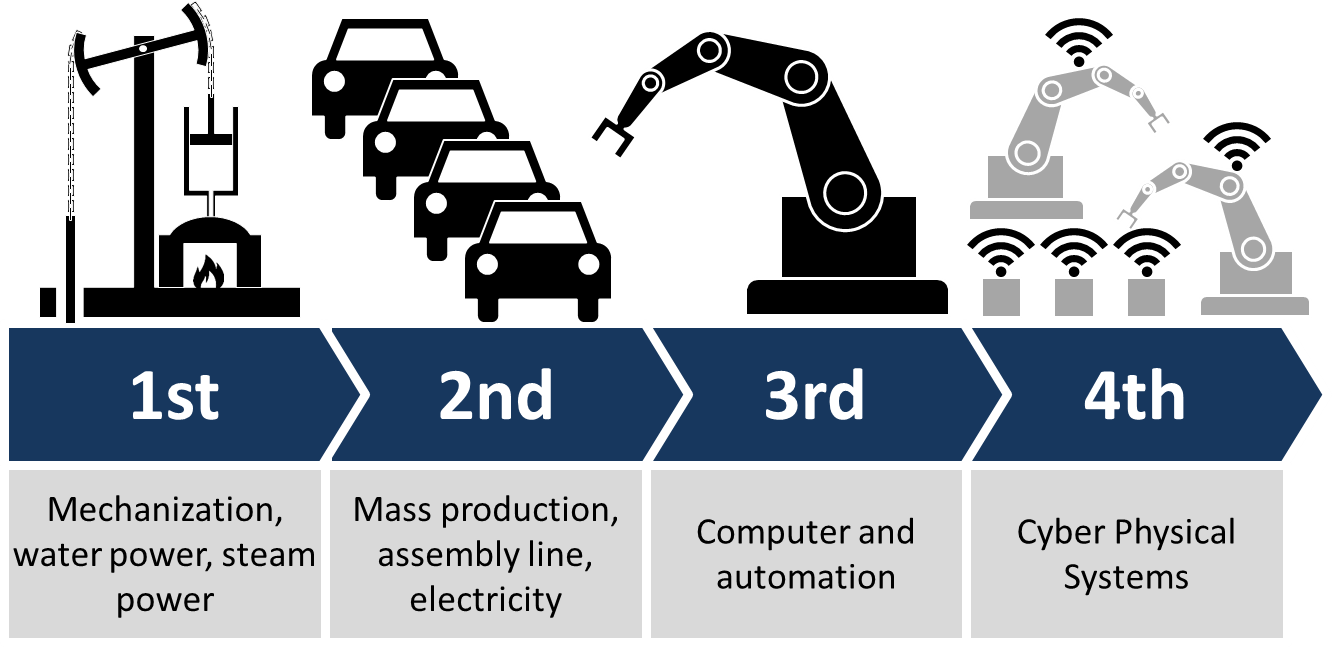
\includegraphics[width=11cm,keepaspectratio]{industry40}
    \caption[The four industrial revolutions that took place over the last centuries]{The four industrial revolutions that took place over the last centuries \autocite{img:industry4.0}}
    \label{fig:industry40}
\end{figure}

This drastic change means that many companies have to adapt to keep up with the competing companies that already have these technologies. Steel belt production companies are no exception. With the invention of a gradient magnetometer that can effectively characterise steel belts, the foundation for this diploma thesis was laid.

\section{Task}

The task of this diploma thesis is to develop a system to read sensor data, process it and visualise the results. Sensor data is continuously read from a highly sensitive MEMS gradient magnetometer. This data is structured as raw binary data and has to be processed by the system. The processed data will also undergo statistical analysis to predict parameters on the basis of this data. After this processing step the data has to be sent wirelessly to a mobile app. This mobile app acts as the client-side of the system. The app visualises the sensor data and its predicted parameters. The app should also offer a way of browsing through historical data that was saved prior.

\subsection{Requirements of GRAMOC}

Server side requirements:

\begin{itemize}
    \item Read data from a sensor
    \item Save sensor data for further inspection
    \item Predict mechanical parameters from sensor data
    \item Send data to clients
    \item Provide historical data to clients
\end{itemize}

Client side requirements:

\begin{itemize}
    \item Visualise sensor data
    \item Provide a form for requesting historical data
    \item Visualise historical data
\end{itemize}

\section{Existing Solutions}

\subsection{Steel Belt Quality Inspection}

Currently there are no solutions for dynamic steel belt characterisation. All these measurements have to be made manually.

The current procedure to inspect the quality of a steel belt is as follows: The first thing that has to be done is to produce a roll of steel belt. To get the quality level of this product, a sample has to be taken from it. There are two samples taken from each steel belt roll, one from the start and one from the end. These two samples can now undergo quality inspection procedures. The results from these tests can be used to assess the produced steel belt. According to these tests, the parameters of the production machines can be adjusted.

This procedure has a few major disadvantages. Firstly, if the product does not pass the quality tests, the whole steel belt has to be discarded. Time and personnel are also two big disadvantages. These quality tests are not only time consuming but they also require special trained staff for conducting these inspections.

\subsection{Handling Sensor Data}

Currently there are a lot of solutions available that can plot sensor data. The majority of these are even free. The one constraint that most of these solutions share is that the sensor has to be directly connected to the computer. As the sensor that is used for this project sends its data over the network, almost all solutions are considered irrelevant. Also some custom features are wanted that these programs do not offer. For example visualizing historical data.

\subsection{Plotting Real Time Data}

\author{Nico Leidenfrost}
%
As already mentioned there are a lot of solutions out there that can be used to plot sensor data. But the one thing that these solutions mostly can not provide is real time plotting. Static plots can be achieved in many different ways, with big amounts of data or just small amounts, many plots combined or divided in separate plots and many more variations are within the bounds of possibility. A lot of these solutions promote themselves with \textit{dynamic data updates} or \textit{streaming data}. That just means that the data can be changed at runtime and therefore some could say the data is displayed in real time. But real time can be defined very differently. As one would say real time applications can update their data once every second, others consider that the data must be updated within less than 20 milliseconds to achieve a high framerate. Most of the solutions available can handle the former definition of real-time but nearly none of them can provide enough performance for the latter. Another important point is the amount of data that one wants to depict, because most of the already existing programs that can handle real-time are just powerful enough to handle small amounts of data.

\section{Outline}

This diploma thesis is structured into two big parts. These parts can be seen as two phases of implementation. Each phase is completely separate. The first phase is a more experimental one as both authors were unfamiliar with these types of projects, so some experience had to be made. At the end of this phase there was a big cut and the project was restarted from the beginning. The second phase discusses the different approaches and decisions that were made starting from this cut. The second phase was not only better planned, but the decisions that were made, were mostly made out of experience from the first phase.

\chapter{Project Management}
\label{ch:Project Management}
There are various projects no matter if it's developing software or even building a bridge, each of them needs to be managed carefully because otherwise it could end with a low quality outcome, time delays or even with enormous costs that the ones running the project can not handle. To prevent all these horrible scenarios project management helps with the application of knowledge, skills, tools and techniques. Project management as it's used and performed nowadays exists since the mid-20th century, but earlier, much simpler versions of it were used since ever.

\section{Kanban}

\subsection{Description of Kanban}
Kanban is a technique to manage software development in a project. It utilizes the just-in-time (JIT) production system and easily reveals possible bottlenecks in the software development pipeline. Kanban provides information in a visual way instead of a textual, therefore the brain can extract information much quicker. The reason is that the human brain is able to processes visual information 60 000 times faster than text \cite{WhatIsKanban}. Kanban uses sticky notes or some sort of cards on a board to display the information. This method packs the pure text information in a bigger picture that the brain can now process faster.

\subsection{How Kanban works}
Kanban has four core principles \cite{WhatIsKanban}.
\begin{enumerate}
    \item \textbf{Visualize Work}

    By visualizing the work and workflow in a project, it's easier to observe the flow of work through the whole Kanban system. Also problems like bottlenecks, blockers and queues can be spotted immediately.

    \item \textbf{Limit Work in Process}

    Kanban limits the amount of unfinished work in process. By doing so it reduces the time one item needs to travel through the Kanban system. That brings the advantage of less task switching and constantly reprioritizing.

    \item \textbf{Focus on Flow}

    By implementing work-in-progress (WIP) limits and team-driven policies the Kanban system can be optimized to improve the workflow. With its methods the flow can be analyzed and it can indicate possible future problems.

    \item \textbf{Continuous Improvement}

    Once the Kanban system is established, teams can track their efficiency by measuring flow, quality and throughput of work items they are assigned to. This can help a team a lot to improve and take their efficiency to a higher level.
\end{enumerate}

\subsection{History of Kanban}
Kanban was developed by Toyota in the late 1940s, the idea of Kanban came up from an unlikely source, the supermarket. They realized that the workers there ordered their goods if the stock was going near zero instead of order more goods if they are available at a vendor. So they ordered their goods after a ``just-in-time'' system. Kanban is Japanese for ``sign'' or ``signboard'', so Toyota invented a system that allowed teams to communicate better and showed them what work is needed to be done and when it's needed \cite{WhatIsKanban}.

\section{Scrum}

\subsection{Description of Scrum}
Scrum is a process framework to control and manage complex software development projects, it reduces the complexity of the whole system and focuses on a product that meets the business needs. ``Scrum makes clear the relative efficacy of your product management and development practices so that you can improve.'' \cite{ScrumGuide}

\subsection{How Scrum works}
Scrum consists of a number of entities that include \cite{WhatIsScrum}:
\begin{itemize}
    \item \textbf{The Scrum Values} originally weren't included in the official Scrum guide, but due to most people considered them as a part of Scrum they were added in July 2016. These values are Commitment, Courage, Focus, Openness and Respect.

    \item \textbf{The Scrum Roles} are three roles every Scrum team needs to consist of. There is the ``Product Owner'', who needs to manage the Product Backlog. He needs to make sure the items are clearly expressed and in an order so that the team can achieve the best possible result. Theres also the ``Scrum Master'', who makes sure Scrum is used and understood properly. He also tells people outside of the Scrum team how they should interact with the team to maximize the output of the team. All of the other members in the Team are part of the ``Development Team''. Such a team is self-organized, cross-functional and there is no particular ranking in the team which means everybody is on the same level. The Development Team and only the Development Team is responsible to complete tasks from the Product Backlog at the end of each Sprint.

    \item \textbf{The Scrum Events} are used to create a regularity and minimize the effort of meetings outside the Scrum meetings. These events all have a fixed timespan and can't be shortened or lengthened. The Events embedded in Scrum are:
    \begin{enumerate}
        \item \textbf{Sprint}

        Each Sprint has a predefined timespan up to one month, in this period of time the Development Team should create a releasable increment to the product. During the Sprint, nobody should make changes that would compromise the goal of the Sprint, also the stated quality of the product does not decrease. The scope of a Sprint can be clarified and re-negotiated with the Product Owner during the Sprint, when a Sprint finishes the next Sprint starts immediately.

        \item \textbf{Sprint Planning}

        The Sprint Planning Event takes place before each Sprint, in this meeting items from the Product Backlog are moved into the Sprint Backlog. These items do not have to be finished in one Sprint as a Sprint is defined by its time limit and not by the items in the Sprint Backlog.

        \item \textbf{Daily Scrum}

        In the Daily Scrum meeting the Development Team creates a plan for the next 24 hours. To do so the attendees analyze the work that has been done so far and with this knowledge they determine what to do until the next meeting. This meeting has a duration of at most 15 minutes and takes place every day in the same place at the same time.

        \item \textbf{Sprint Review}

        This meeting is held at the end of each Sprint, its purpose is to analyze the outcome and what items in the Sprint Backlog were actually finished in this Sprint. Attendees of this meeting are the Scrum team and the stakeholders, both groups should collaborate on the next things that could be done.

        \item \textbf{Sprint Retrospective}

        The main focus in this particular meeting lays on the improvement that can be done during the next Sprint. The topics discussed in the Sprint Retrospective are ``What went well in the Sprint'', ``What could be improved'' and ``What will we commit to improve in the next Sprint''.
    \end{enumerate}

    \item \textbf{Scrum Artifacts} represent the work that is to do or already is done to make it easier to inspect and adapt the particular work units. Therefore there are three Artifacts, the first one is the \emph{Product Backlog}, here defined are requirements that might be needed in the product. The Product Backlog evolves with the product itself, there will be requirements added and removed based on the results of the Sprints finished. The second Artifact is the \emph{Sprint Backlog}, in here are items that are assigned to do in the corresponding Sprint plus a plan how to accomplish the Sprint goal. The last Artifact is the \emph{Increment}, this is described as the sum of all items in the Product Backlog that are finished within the Sprint.
\end{itemize}

\section{Scrumban}

\subsection{Description of Scrumban}
The term ``Scrumban'' is a composition of the two terms ``Scrum'' and ``Kanban'', therefore Scrumban is a project management technique mix of Scrum and Kanban. Scrumban takes the best of both management systems and combines them into one powerful tool to help teams develop their products even faster than before.

\subsection{How Scrumban works}
Scrum is based on fixed time windows called Sprints and the communication between the people delivering the product, Kanban however is based on fixed pieces of work and showing when they need to be done. So Scrumban takes the workpiece based Kanban system and adds the communicational aspects of scrum.

\subsection{Application of Scrumban in this Project}
Scrumban was chosen to be applied in this project because it fitted the already used project management methods. With this technique the tasks could be finished even faster than before and even with a higher quality result. There were meetings as defined within Scrum and a couple of Kanban-boards assigned to the proper members of the team.


\part{Implementationphase 1}
\chapter{Networking Technologies}
\label{ch:networkingtechnologies}

\author{Nico Kratky}
%
\section{Networking in GRAMOC}

Because GRAMOC is based on basic a client-server architecture, a common way of communication had to be developed. This development process resulted in GSDEP.

\section{GSDEP}

GRAMOC Sensor Data Exchange Protocol (GSDEP) is GRAMOC's Network Protocol that is used for sending large amounts of sensor data to the clients. It is built on top of the TCP/IP stack \cite{rfc793, rfc791}.

\subsection{Data Flow}
\label{sec:networking_data-flow}

Figure \ref{fig:handshake} depicts the handshake performed by GSDEP that is based on TCP's three-way handshake. The Client sends a synchronize (SYN) message to the server to let it know that it wants to connect. If the server can accept new Clients it returns an acknowledgment message (ACK). The client then also returns this acknowledgment message to inform the server that it is indeed connected. The connection now is established.

\begin{figure}[H]
    \centering
    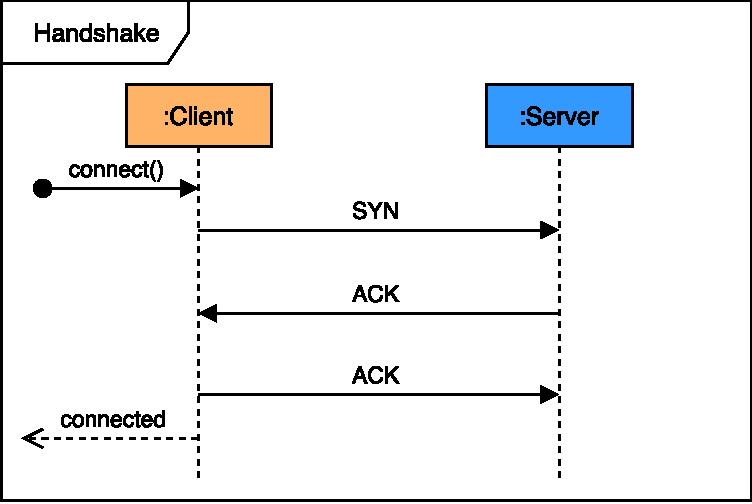
\includegraphics[width=8cm,keepaspectratio]{gsdep_handshake}
    \caption{TCP-like three way handshake performed on client connect}
    \label{fig:handshake}
\end{figure}

If a client wants to disconnect from the server it will send a disconnect message (FIN) to the server. Before it actually disconnects, it has to wait for the server to finish cleaning up and return the FIN packet. After the client has received this message, it can close the connection and shut down. This procedure is shown in Figure \ref{fig:disconnect}.

\begin{figure}[H]
    \centering
    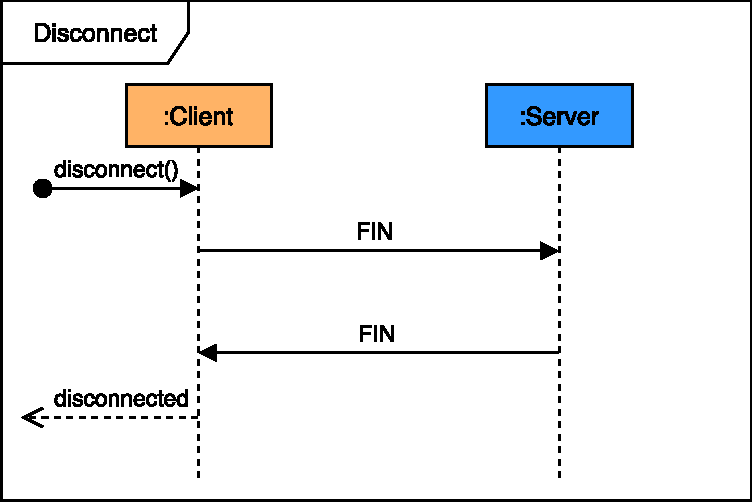
\includegraphics[width=8cm,keepaspectratio]{gsdep_disconnect}
    \caption{Two way handshake performed on client disconnect}
    \label{fig:disconnect}
\end{figure}

\subsection{Data Interchange Format}

Every message is made up of a header and the actual payload that will be transmitted. The header includes additional information that is used by the receiving end to determine the size of the payload (see \ref{sec:messageframing}), to differentiate between different kinds of messages (see \ref{sec:channels}) and to rebuild the message data to its correct data type. As depicted in Figure \ref{fig:packet}, the header consists of 4 bytes message length and 2 bytes each for data type and channel.

\begin{figure}[H]
    \centering
    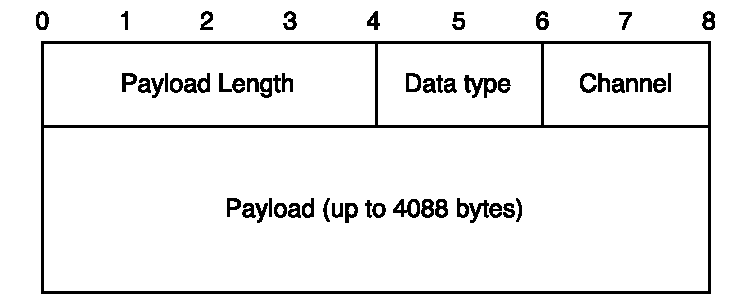
\includegraphics[width=8cm,keepaspectratio]{gsdep_packet}
    \caption{Structure of one packet sent by GSDEP}
    \label{fig:packet}
\end{figure}

\subsection{Commands}
\label{sec:networking_command}

Commands are special messages that require further action to be taken. These commands can either be used during the connect or disconnect handshakes, or to request data.

\begin{table}[H]
    \centering
    \begin{tabular}{| l | l | p{5cm} |}
    \hline
    \textbf{Command} & \textbf{Used by} & \textbf{Meaning} \\ \hline
    SYN & client & Tells the server that a new client is waiting for the connection procedure \\ \hline
    ACK & server \& client & Tells the other end that it acknowledges the previous command \\ \hline
    FIN & server \& client & Tells the other end that it will disconnect \\ \hline
    STD & client & Tells the server that a client requests data\\ \hline
    SPD & client & Tells the server that a client does not want any more data\\
    \hline
    \end{tabular}
    \caption{Commands sent by one of the connection partners and what they do}
    \label{tab:commands}
\end{table}

\subsection{Channels}
\label{sec:channels}

In the case of GRAMOC, where large amounts of data are received in short periods of time, it is crucial to differentiate between communication data and sensor data in split seconds. To accomplish this a 2 byte unsigned short is included in the packet header. This information can the be used to tell apart these two types of data.

\begin{table}[H]
    \centering
    \begin{tabular}{| l | c |}
    \hline
    \textbf{Channel} & \textbf{Value} \\ \hline
    Communication & 1 \\ \hline
    Data & 2 \\
    \hline
    \end{tabular}
    \caption{Channels used to distinguish between message types}
    \label{tab:channels}
\end{table}

\subsection{Message framing}
\label{sec:messageframing}
Because TCP operates with streams of data and not packets of data, messages have to be framed so that the receiving end knows what one message is. This can be achieved in two ways. \cite{MessageFramingCleary,MessageFramingSkotzko}

\subsubsection{Length Prefixing}

One method of message framing is to prefix each message with its length. When doing so the format of this prefix has to be stated explicitly. In the case of GSDEP that is a ``4 byte unsigned integer''.

\paragraph{Sending}

First, the message has to be encoded into its binary representation. To send this message, the length followed by the binary encoded message simply has to be sent.

\paragraph{Receiving}

Receiving one message is done by first reading into a buffer with the length of the length prefix (in this instance the buffer would be 4 bytes long). Then the payload is read into a second buffer with the just read length. When this buffer is full, one message has been read.

\subsubsection{Delimiters}

\paragraph{Sending}

Messages can also be framed by using delimiters. This can be done by sending a special character between each message. This character can either be a character that does not show up in actual messages (e.g. a Null character), or a character that is present in a message. If the second approach is used, every message has to be run through an escaping process which replaces these characters in the messages.

\paragraph{Receiving}

Receiving delimited messages is relatively straightforward. One message is read when a delimiter is reached. This message has to be passed to an unescaping function when a delimiter character is chosen that can exist in messages.

\subsubsection{Security Concerns}

Whichever solution is chosen, each solution has to provide code regarding Denial of Service (DoS) attacks. Wether a very big message length or large amounts of data without a delimiter are received, both can result in Out of Memory Exceptions.

\chapter{Server}
\label{ch:server}

\author{Nico Kratky}
%
A server is a computer program that supplies clients with services. The term 'server' often refers to the machine on which the program is running on. In this project the server has to accomplish several tasks. It has to read data from the sensor that is used, and distribute this data to clients. To do this it also has to manage clients and incoming connection requests.

\section{Hardware}
\todo{Put something here}
\subsection{Raspberry Pi 3 Model B}
% The Raspberry Pi is a small single-board computer originally created to teach children how to program \autocite{RasPi}. It was developed by the Raspberry Pi Foundation. There are numerous options for expanding the capabilities of the Raspberry Pi. One being the use of General-purpose input/output (GPIO) pins. They can be used to connect so-called HAT's (Hardware Attached on Top) or Shields (this term evolved from Arduino-land). These add-on boards are mounted to the Raspberry Pi by connecting the GPIO pins to the board and screwing them together. They mostly provide additional hardware to extend the application possibilites and to achieve the desired goal. Further advantages are its relatively small footprint and its low cost. Also, a wide variety of Linux distributions have been adapted to the hardware. Having these advantages was the decisive factor for choosing the Raspberry Pi 3 Model B.\\
% The specifications of the Raspberry Pi 3 Model B are:

The Raspberry Pi is a small single-board computer, developed by the Raspberry Pi Foundation \autocite{RasPi}. Originally it was created to teach children how to use computers and more importantly, how to program them. The biggest advantage of these mini-computers is the variety of extension possibilities. These extension are so-called HAT's (Hardware Attached on Top) or Shields (which is a term that is more often used when talking about Arduinos). They are connected by using the on-board General-purpose input/output (GPIO) pins. They mostly provide additional hardware to extend the application possibilities and to achieve the desired goal. Further advantages are its relatively small footprint, low cost and wide-variety of available Linux distributions. Having these advantages was the decisive factor for choosing the Raspberry Pi. In this project the latest available version, which is the Raspberry Pi 3 Model B, was used. Specifications of this computer are listed in table \vref{tab:raspispec}.

\begin{minipage}{\textwidth}
\begin{table}[h]
    \centering
    \begin{tabularx}{\linewidth}{| l | X |}
    \hline
    \textbf{SoC} & Broadcom BCM2837 \\ \hline
    \textbf{CPU} & 4x ARM Cortex-A53, 1.2GHz \\ \hline
    \textbf{GPU} & Broadcom VideoCore IV \\ \hline
    \textbf{RAM} & 1GB LPDDR2 (900MHz) \\ \hline
    \textbf{Networking} & 10/100 Ethernet, 2.4GHz 802.11n wireless \\ \hline
    \textbf{Bluetooth} & Bluetooth 4.1 Classic, Bluetooth LE \\ \hline
    \textbf{Storage} & microSD \\ \hline
    \textbf{GPIO} & 40-pin header, populated \\ \hline
    \textbf{Ports} & HDMI, 3.5 analogue audio-video jack, 4x USB 2.0, Ethernet, Camera Serial Interface (CSI), Display Serial Interface (DSI) \\ \hline
    \end{tabularx}
    \caption{Raspberry Pi 3 Model B specifications}
    \label{tab:raspispec}
\end{table}
\end{minipage}

\begin{figure}[H]
	\centering
	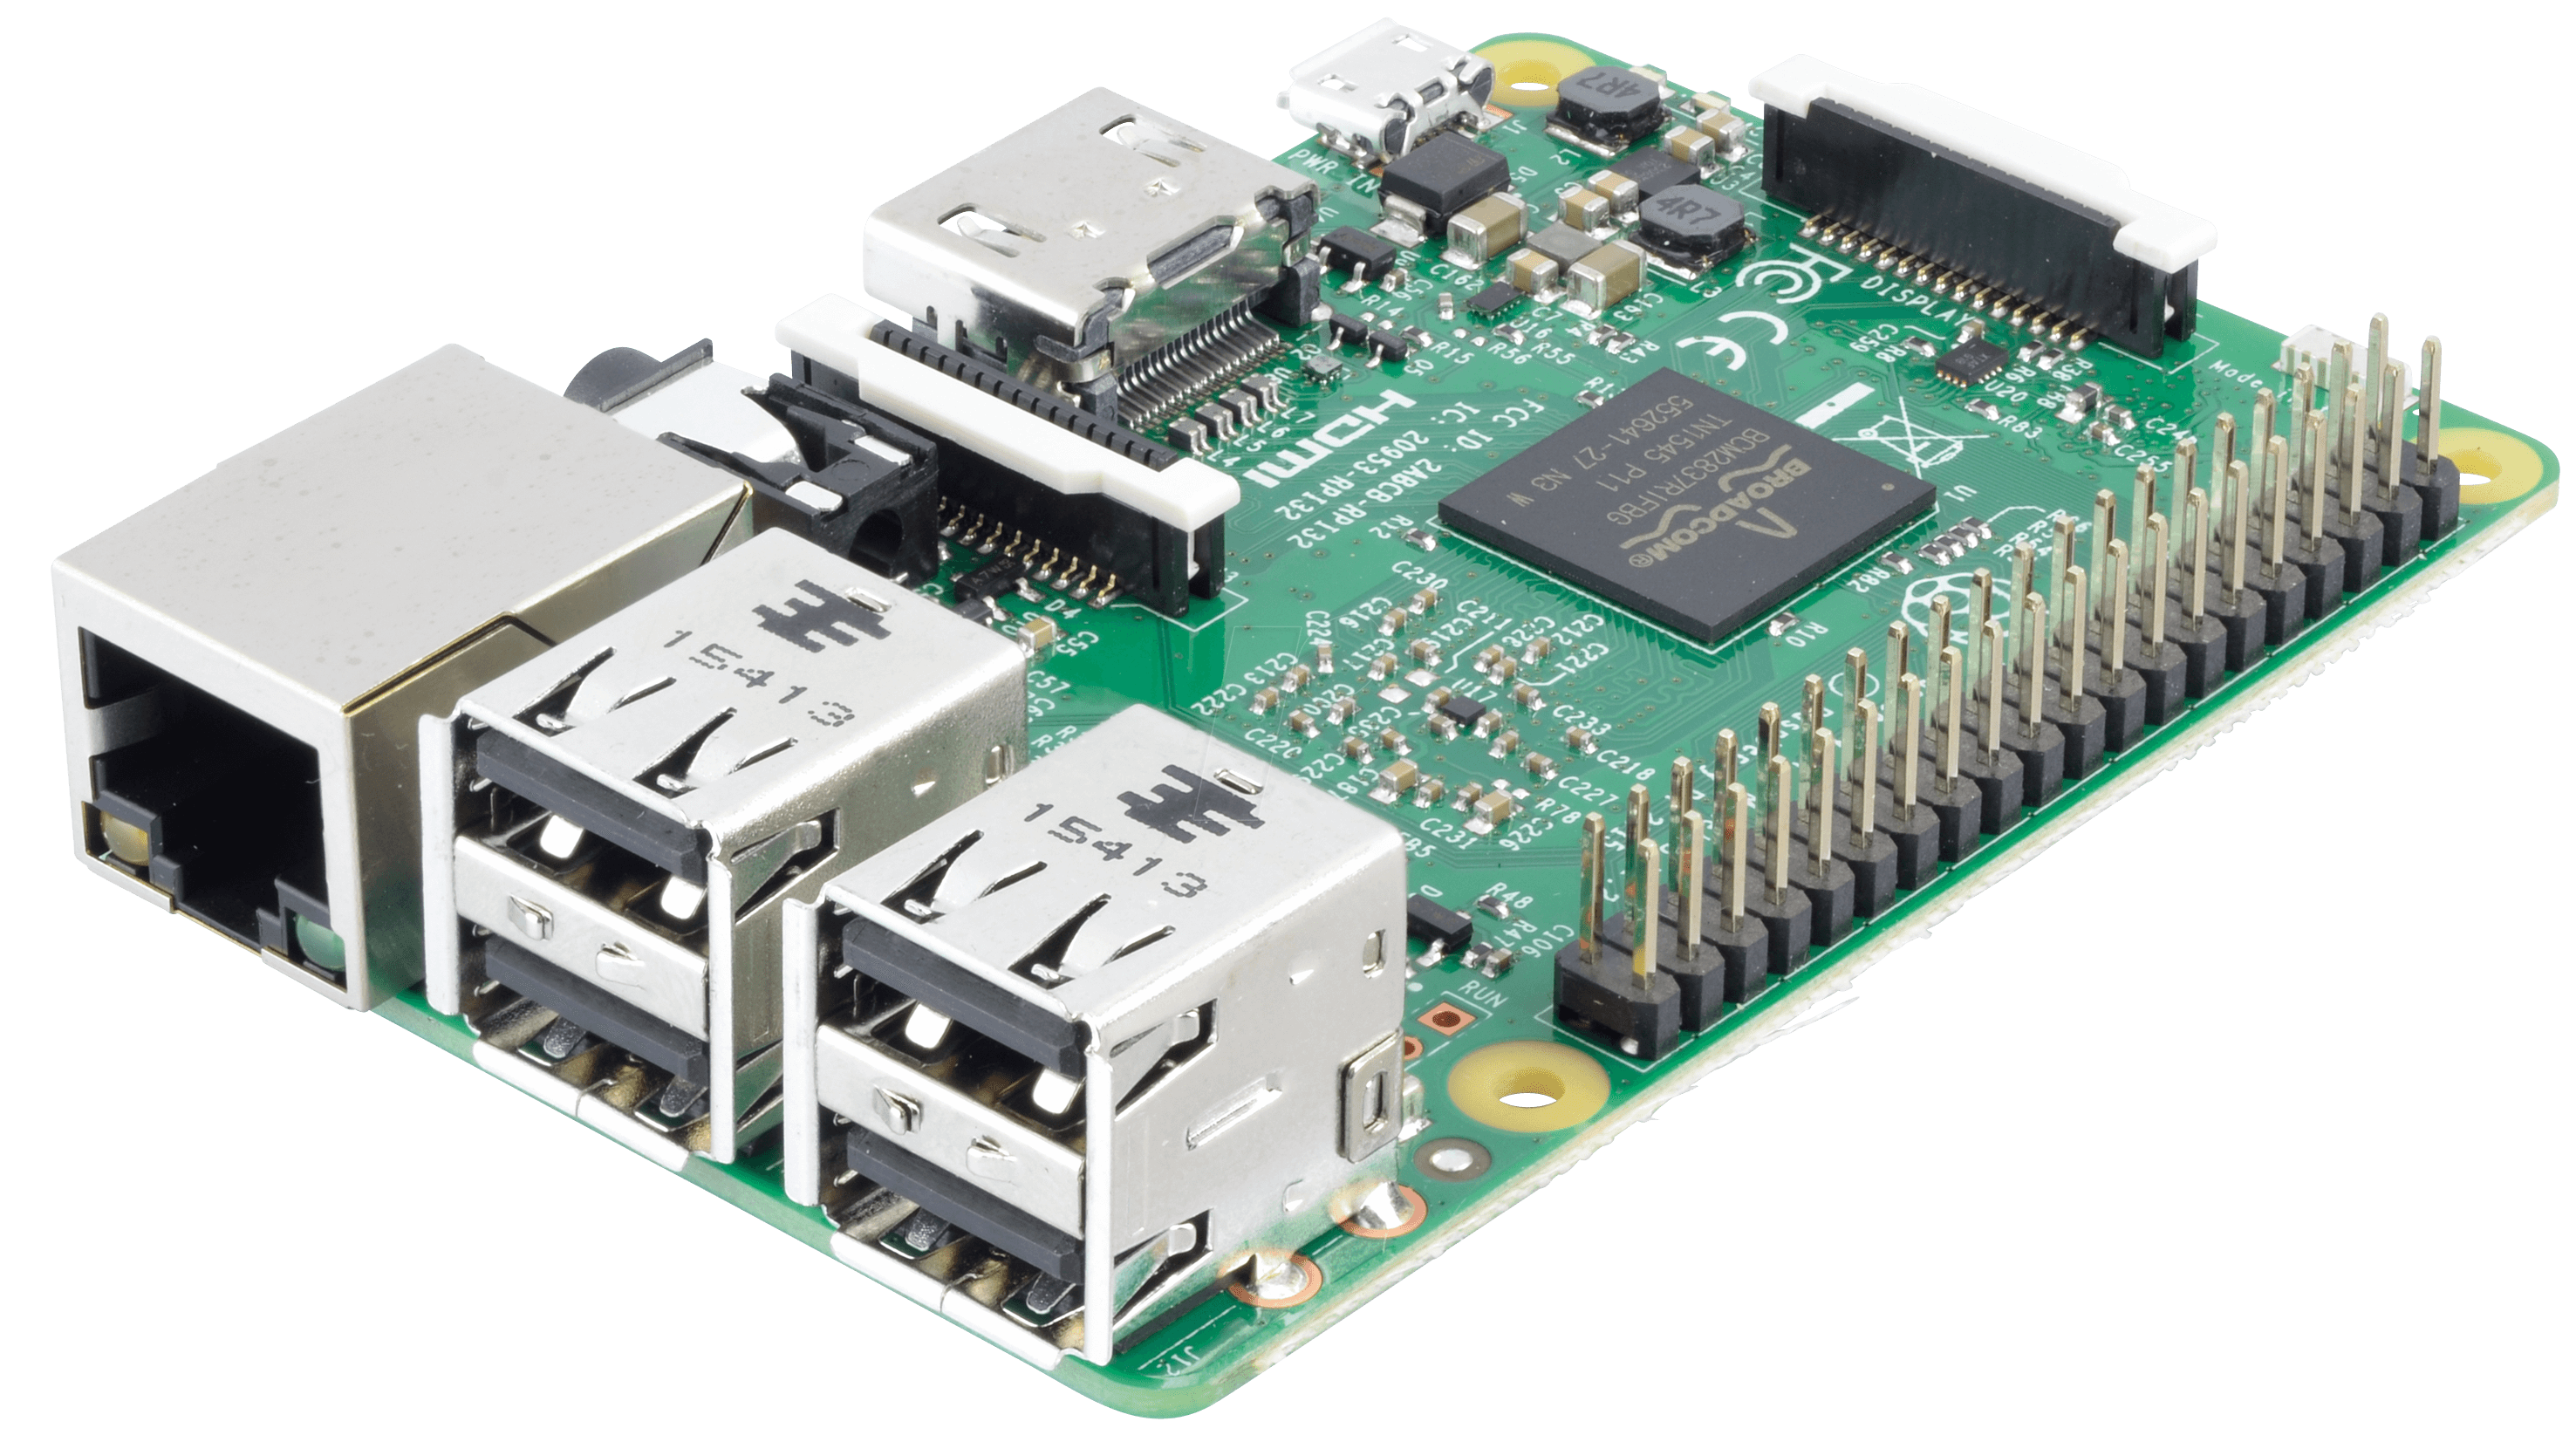
\includegraphics[width=10cm,keepaspectratio]{raspberrypi3b}
	\caption[Raspberry Pi 3 Model B]{Raspberry Pi 3 Model B\footnotemark}
	\label{fig:raspberrypi3b}
\end{figure}

\footnotetext{\cite{img:raspi}}

\subsection{Raspberry Pi SenseHAT}

The SenseHAT was made especially for the Astro Pi mission, where student could create and code projects, which were then run on the International Space Station by astronaut Tim Peake \autocite{AstroPiMission}. This board was chosen because it offers a wide variety of sensors and therefore offers many possibilities in terms of testing GRAMOC. Figure \vref{fig:sensehat} shows a SenseHAT that is not attached to a Raspberry Pi.

The Raspberry Pi Sense HAT includes following sensors and inputs/outputs \autocite{SenseHAT}:

\begin{itemize}
	\item ST LSM9DS1 Inertial measurement sensor
		\begin{itemize}
			\item 3D accelerometer
			\item 3D gyroscope
			\item 3D magnetometer
		\end{itemize}
	\item ST LPS25H barometric pressure and temperature sensor
	\item ST HTS221 relative humidity and temperature sensor
	\item Alps SKRHABE010 5-button mini-joystick
	\item 8x8 RGB LED matrix
\end{itemize}

Although GRAMOCs main task is to charactarize steel belts using a magnetometer, a Raspberry Pi SenseHAT add-on board was used to get sensor data. It was dicided to use the now available accelerometer to perform measurements because it's easier to control the sensor data than by using the magnetometer. Different sensor values can be generated by simply moving around the Raspberry Pi with the attached SenseHAT.

\begin{figure}[H]
	\centering
	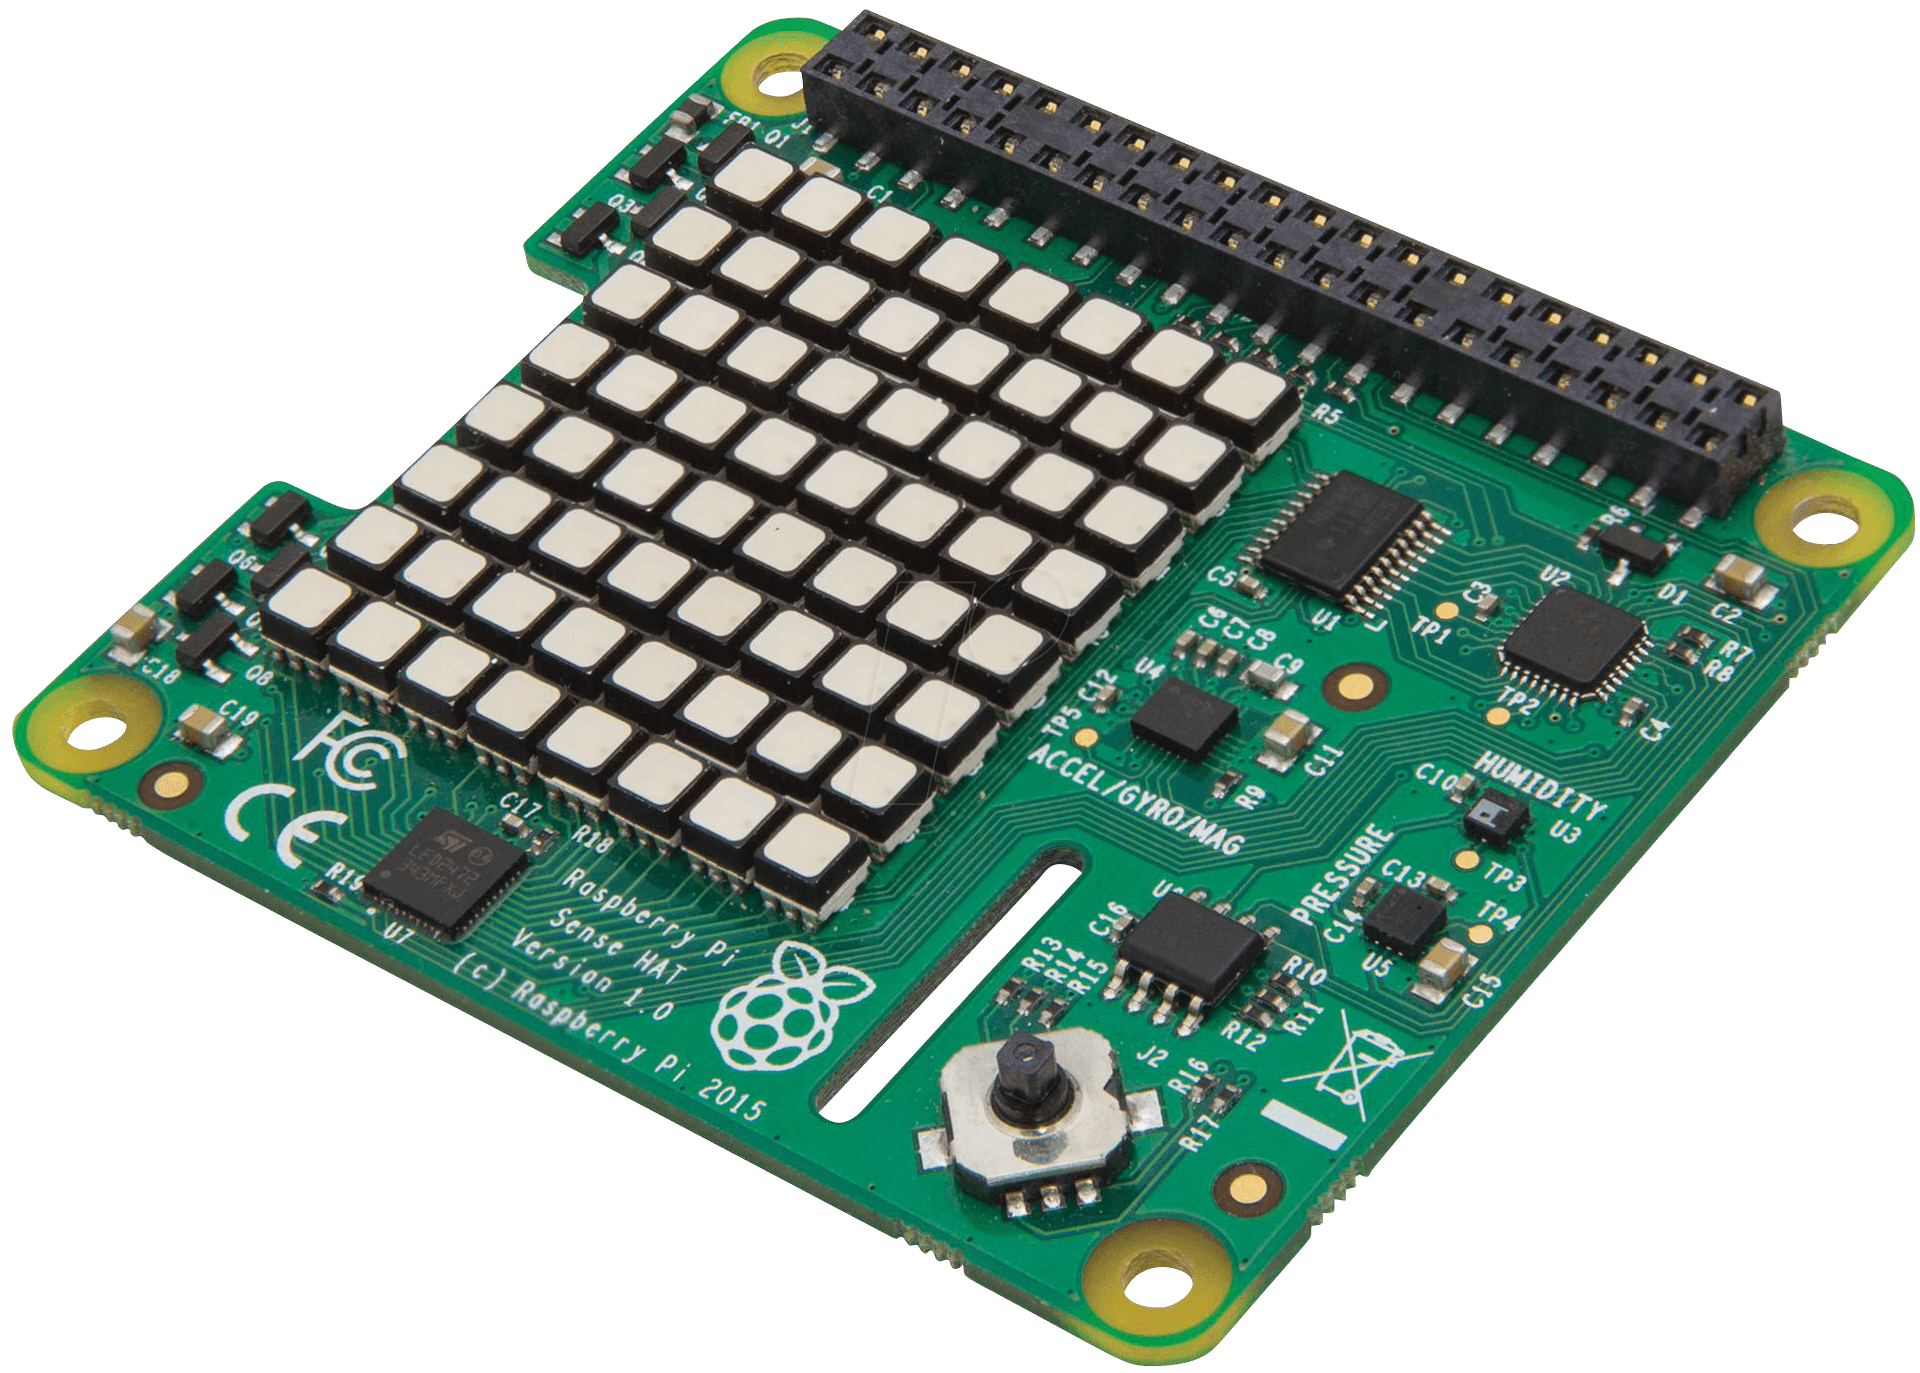
\includegraphics[width=8cm,keepaspectratio]{sensehat}
	\caption[Raspberry Pi SenseHAT]{Raspberry Pi SenseHAT\footnotemark}
	\label{fig:sensehat}
\end{figure}

\footnotetext{\cite{img:sensehat}}

\section{Implementation}

The server program of GRAMOC is completely written in Python. This allows for great compatibility as Python comes preinstalled on many systems.

\subsection{Programming Language}

Python is a simple yet powerful, modern programming language and supports both procedure-oriented as well as object-oriented programming. It was developed by Guido van Rossum at Centrum Wiskunde \& Informatica (CWI) in the Netherlands in 1989 and first released in 1991 \autocite{HistoryOfPython}. It was meant to be a successor to the ABC programming language. Python is a high-level language and therefore includes features such as automatic memory management.

Python is currently available in version 3.6.2. Nevertheless version 2.7 is still available as the Python Software Foundation announced that it will be supportet until 2020, effectivly making it an Long-term support version. Despite that, Python 3.6.2 was chosen for GRAMOC as the Foundation also encourages users to use the newest version if possible. Another reason for choosing the newer version is that GRAMOC does not have to be backwards compatible to any existing software.

\section{Program Flow}

As depicted in figure \vref{fig:server-program-flow}, the server starts accepting new connections right after is has started. It then performs the handshake that is required by GSDEP (further explained in \vref{sec:networking_data-flow}). If this handshake is performed without errors, the server starts listening for data from this now connected client on a separate thread. While this thread is running it receives one message and checks if it is a command (see \vref{sec:networking_command}). If it is, the message is interpreted and the appropriate function is executed. This thread is kept alive until the client disconnects or the server is shutdown by the user.

\begin{figure}[H]
	\centering
	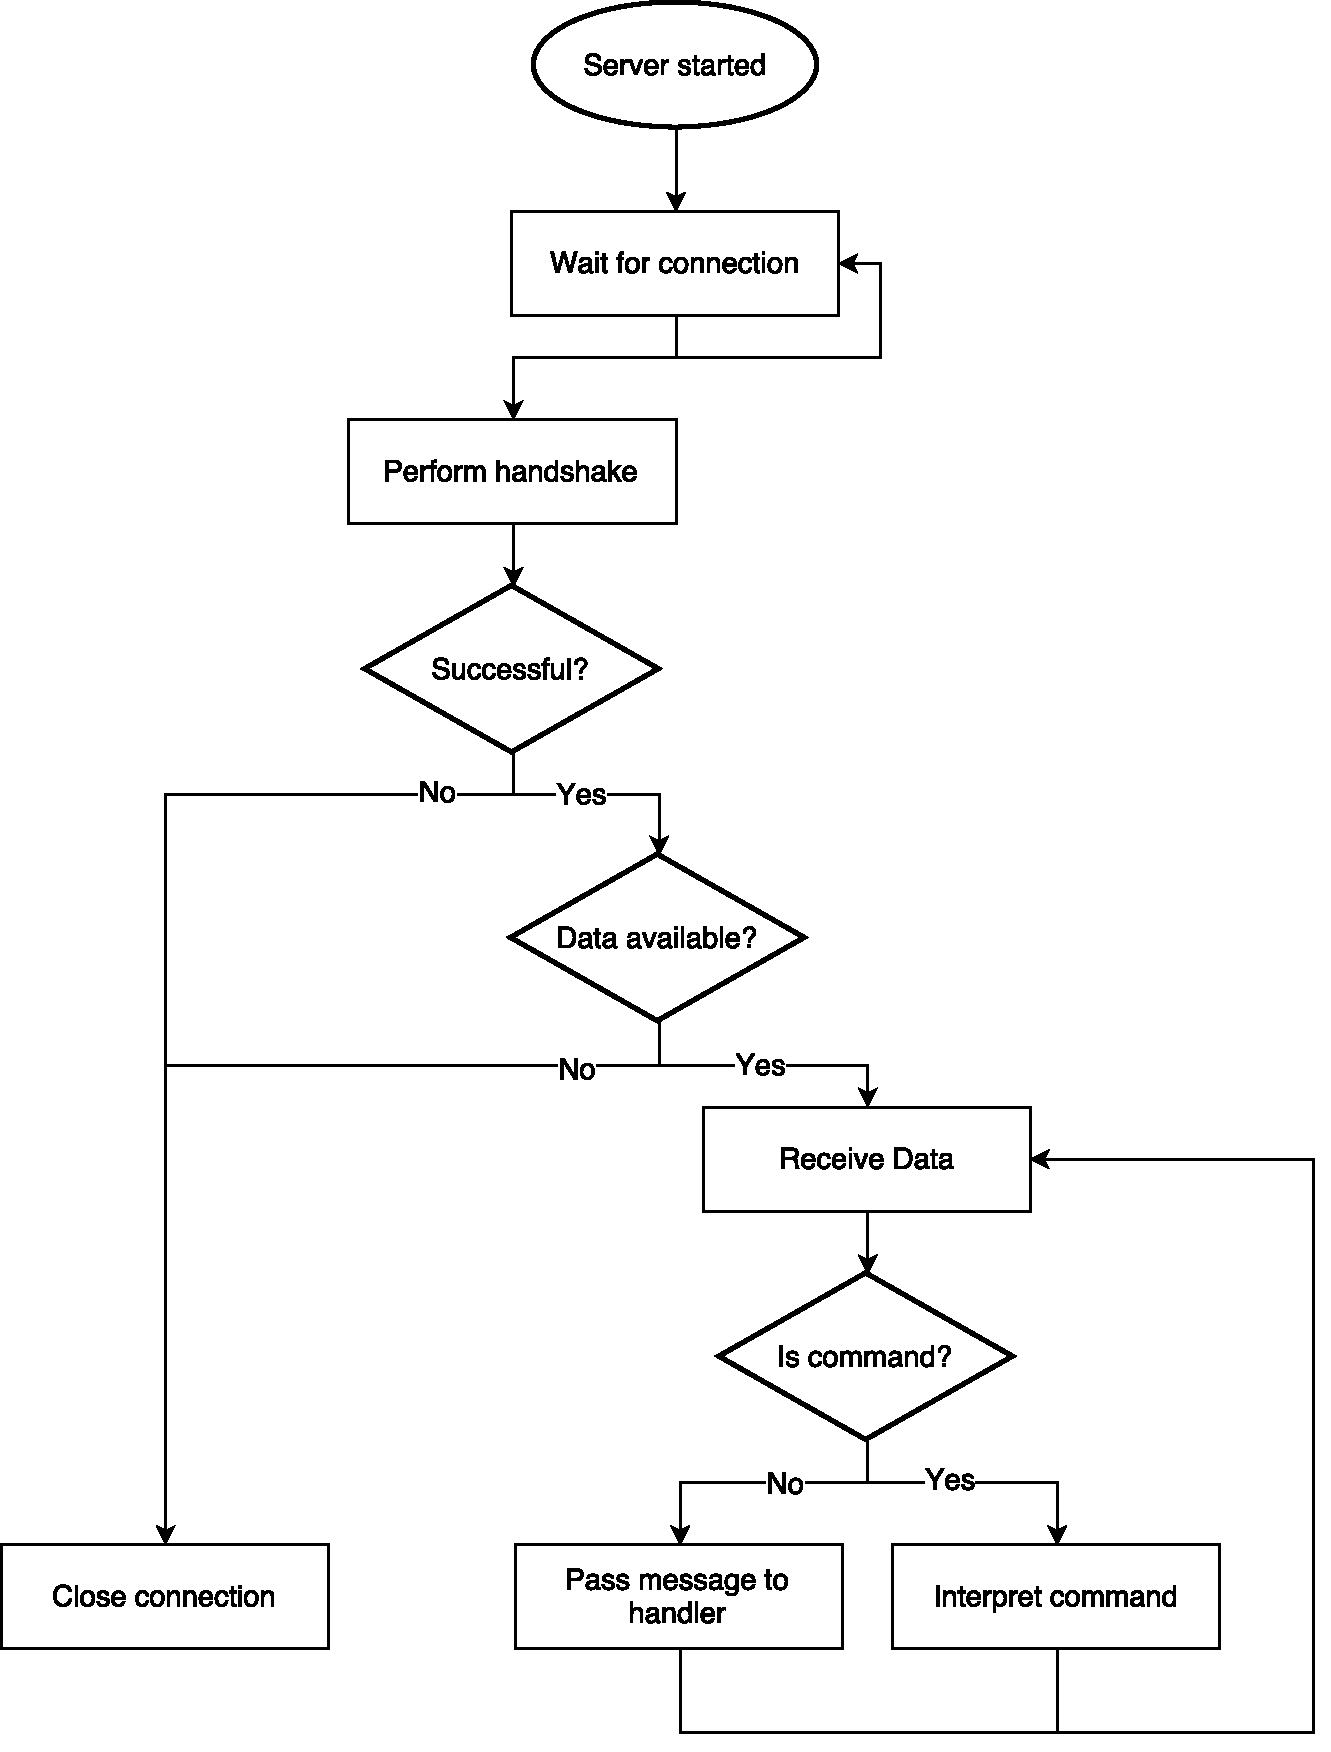
\includegraphics[width=13cm,keepaspectratio]{server-task}
	\caption{Flowchart of server program showing the procedure}
	\label{fig:server-program-flow}
\end{figure}

\chapter{Android}
\label{ch:Android}
Android is a mobile operating system developed by Google, based on the Linux kernel. Android's primary focus is on mobile handheld devices with a touchscreen. The most popular examples would be smartphones, tablets and everything in between, like phablets. Android is open source which means developers can modify the underlying operating system as they wish. Android programs are called ``apps'' which is the short version of application, these applications extend the basic functionality of an Android device.

\section{History of Android}
Android started as a startup Company under the name ``Android Inc.'' It was founded in Palo Alto, California in October 2003. It was meant to be an advanced operating system for digital cameras. In 2004 they changed their goals to expand their operating system to handheld devices that can compete against Symbian and other mobile operating systems which were state of the art at this time. In July 2005 Google bought the whole company along with its key employees for a huge amount of money, 50 Million U.S. dollar at least, according to rumors. They developed a prototype which had similarities with a BlackBerry phone, it had no touchscreen and a physical QWERTY keyboard. Due to the launch of the Apple iPhone in 2007, Google changed its Android specification documents to state that "Touchscreens will be supported", although "the Product was designed with the presence of discrete physical buttons as an assumption, therefore a touchscreen cannot completely replace physical buttons". The first commercially available smartphone using Android as its operating system was the HTC Dream announced in 2008. Since then Google launched numerous updates which improved the operating system bit by bit. They fixed bugs from prior releases and added new features along the way. Android major versions also have a naming scheme, they are all named after a dessert or a sugary treat. Each version starting with the next character in the alphabet starting with version 1.5 called ``Cupcake'', followed by 1.6 as ``Donut'' up to 7.0 as ``Nougat'' and the current version 8.0 as ``Oreo''. Google explained this naming scheme with the following sentence ``Since these devices make our lives so sweet, each Android version is named after a dessert''.

\section{Overview of Android Application Development}
 Applications are often abbreviated as ``apps''. These Android apps are written using the Android software development kit (SDK). There are a small selection of programming languages available that can be used to develop a native Android app.

\subsection{Java}
Java is the most popular language to develop an Android application. The majority of apps and libraries are written in Java. These apps are compiled to bytecode for the Java virtual machine, which is then translated to Dalvik bytecode. The Dalvik virtual machine is a process virtual machine developed for the Android platform. Since Android 5.0 Dalvik is discontinued and the Android Runtime was introduced, which now translates the application's bytecode into native instructions.

\subsection{C/C++}
With C or C++ Code and the Android native development kit (NDK), a native library for Android, applications can get much better results in terms of performance. Because the C or C++ Code runs natively on the device it executes faster than the Java code run in the Android runtime environment. The only downside of this is that all of the C or C++ code needs to be handled through the Java native interface (JNI). This programming framework handles the interoperability of the Java code and the C/C++ Code.

\subsection{Go}
The Go programming language is an open source project developed by a team at Google and many contributers from the open source community \cite{GoProject}. This programming language is supported although there are limitations to the application programming interfaces (API).

\subsection{Kotlin}
In May 2017, Google announced official support for the Kotlin Programming language. Kotlin is a modern and powerful language and solved some issues addressed with Java (e.g. Null references). Kotlin is also interoperable with Java which means Kotlin can be used in already existing Java projects.

\section{Design}
Material Design is Google's visual design language that was first introduced in 2014. The goal was to develop a single underlying system that allows for a unified experience across all kinds of devices. It tries to support visual elements with the characteristics of real materials, hence Material Design. These guidelines help the users to interact and quickly understand different kinds of User Interface (UI) elements by using familiar tactile attributes.

GRAMOC's Android app uses these design principles for the user interface as shown in figure \ref{fig:appscreenshots}

\begin{figure}[H]
	\centering
	\begin{tabular}{cc}
	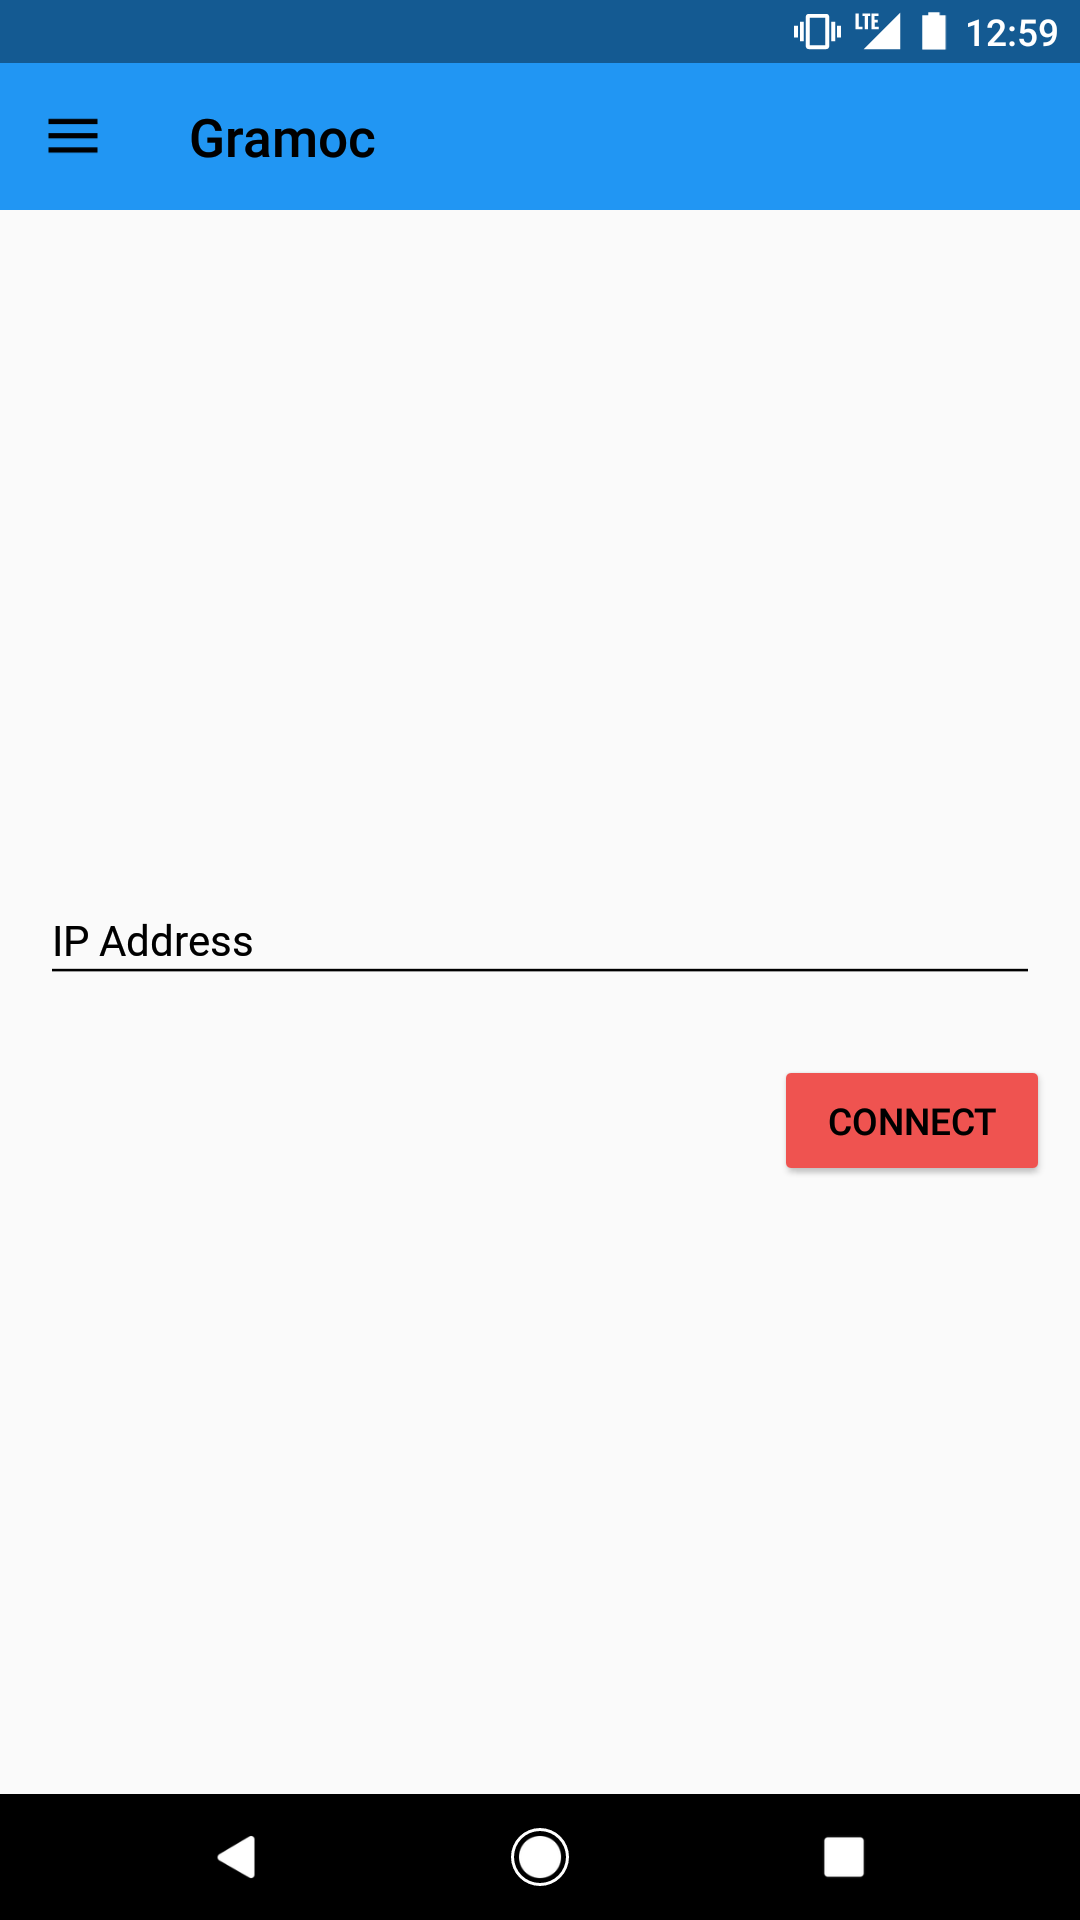
\includegraphics[height=7cm,keepaspectratio]{app_connect}
	&
	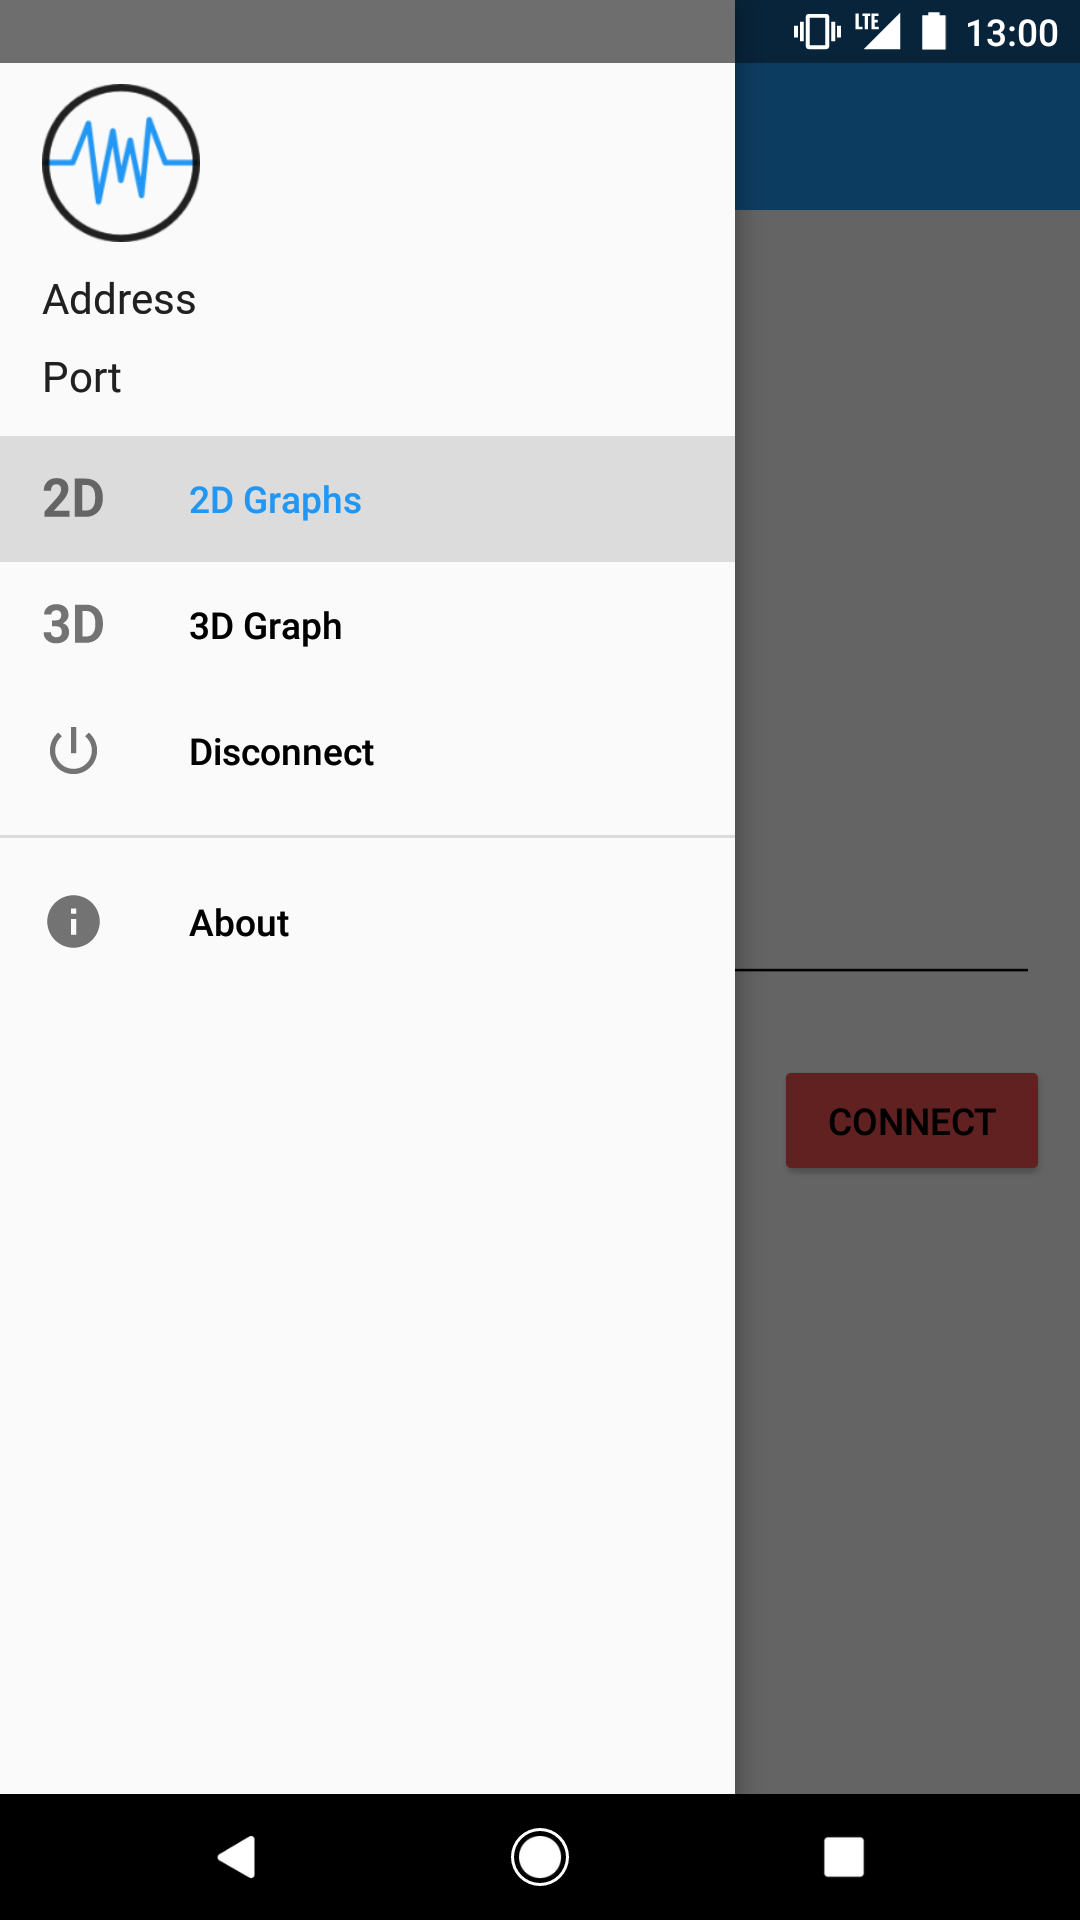
\includegraphics[height=7cm,keepaspectratio]{app_navdrawer}
	\\
	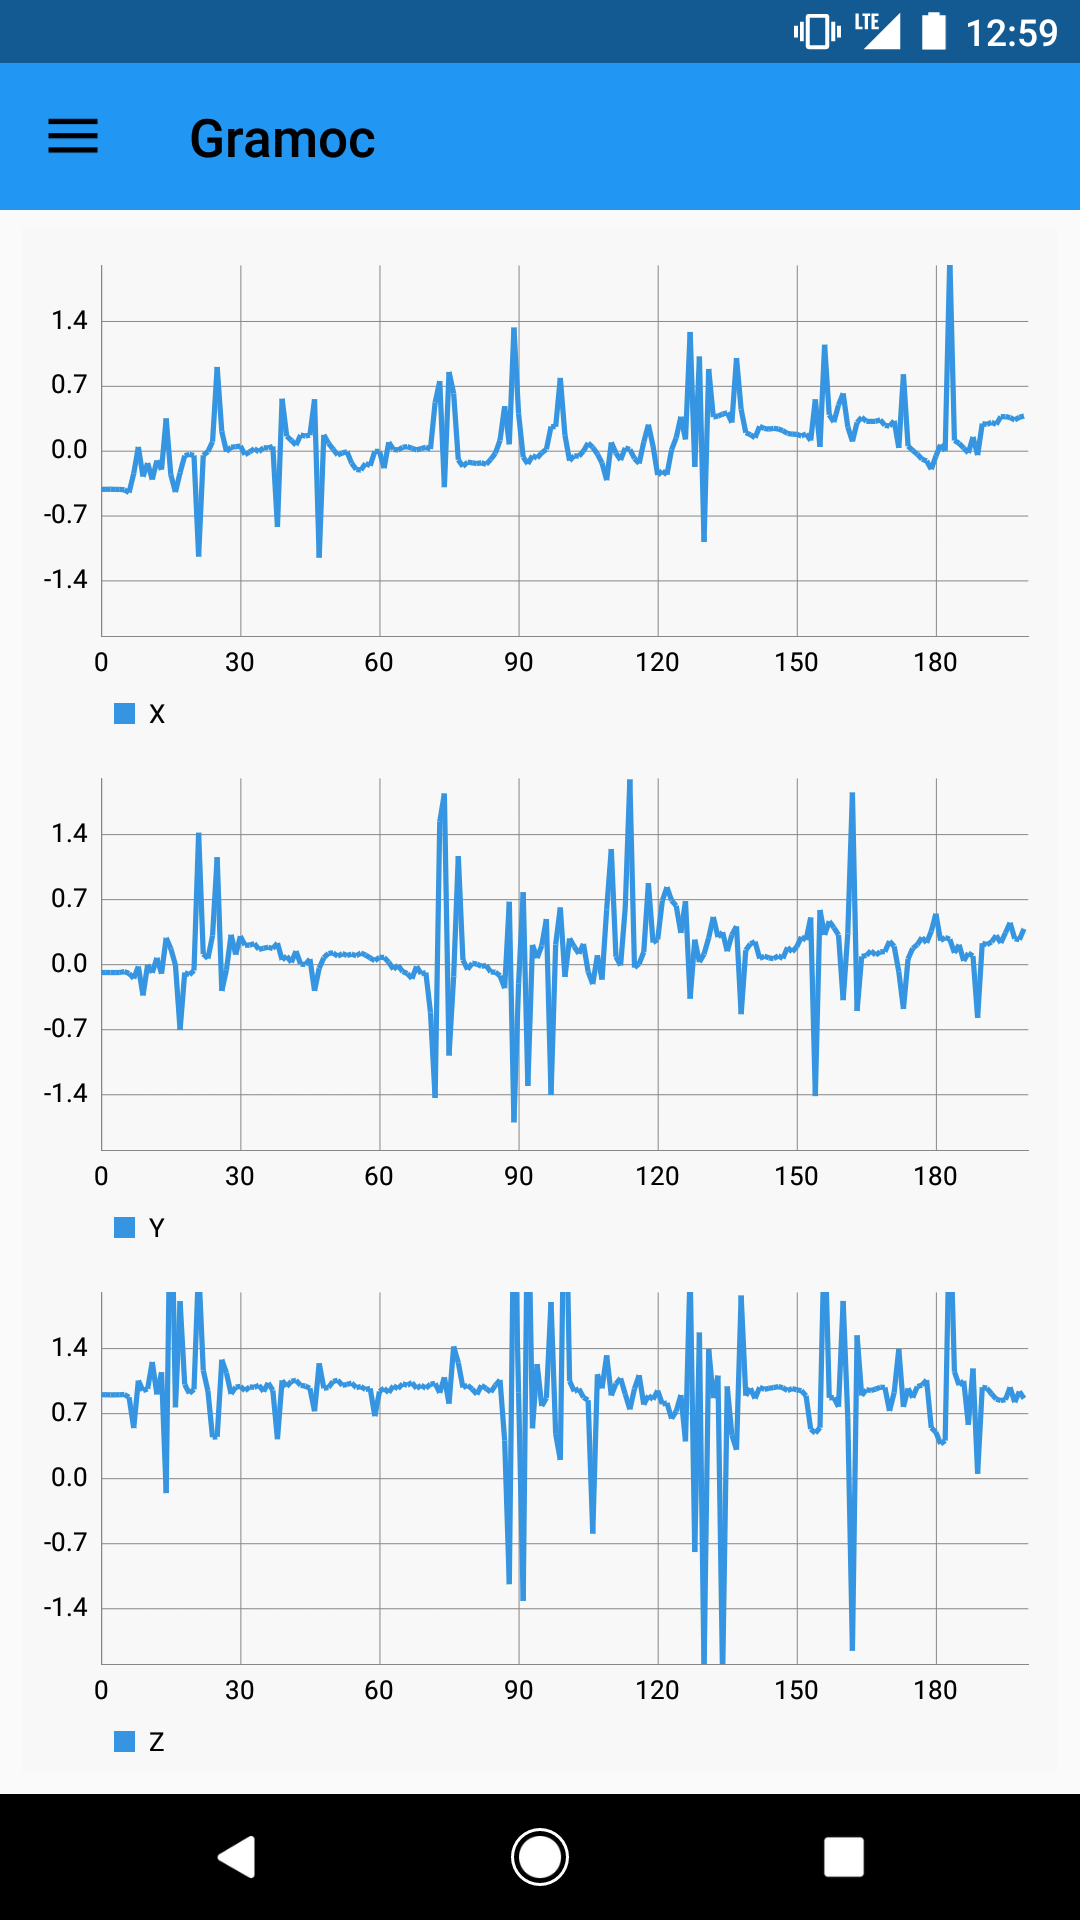
\includegraphics[height=7cm,keepaspectratio]{app_sensor}
	&
	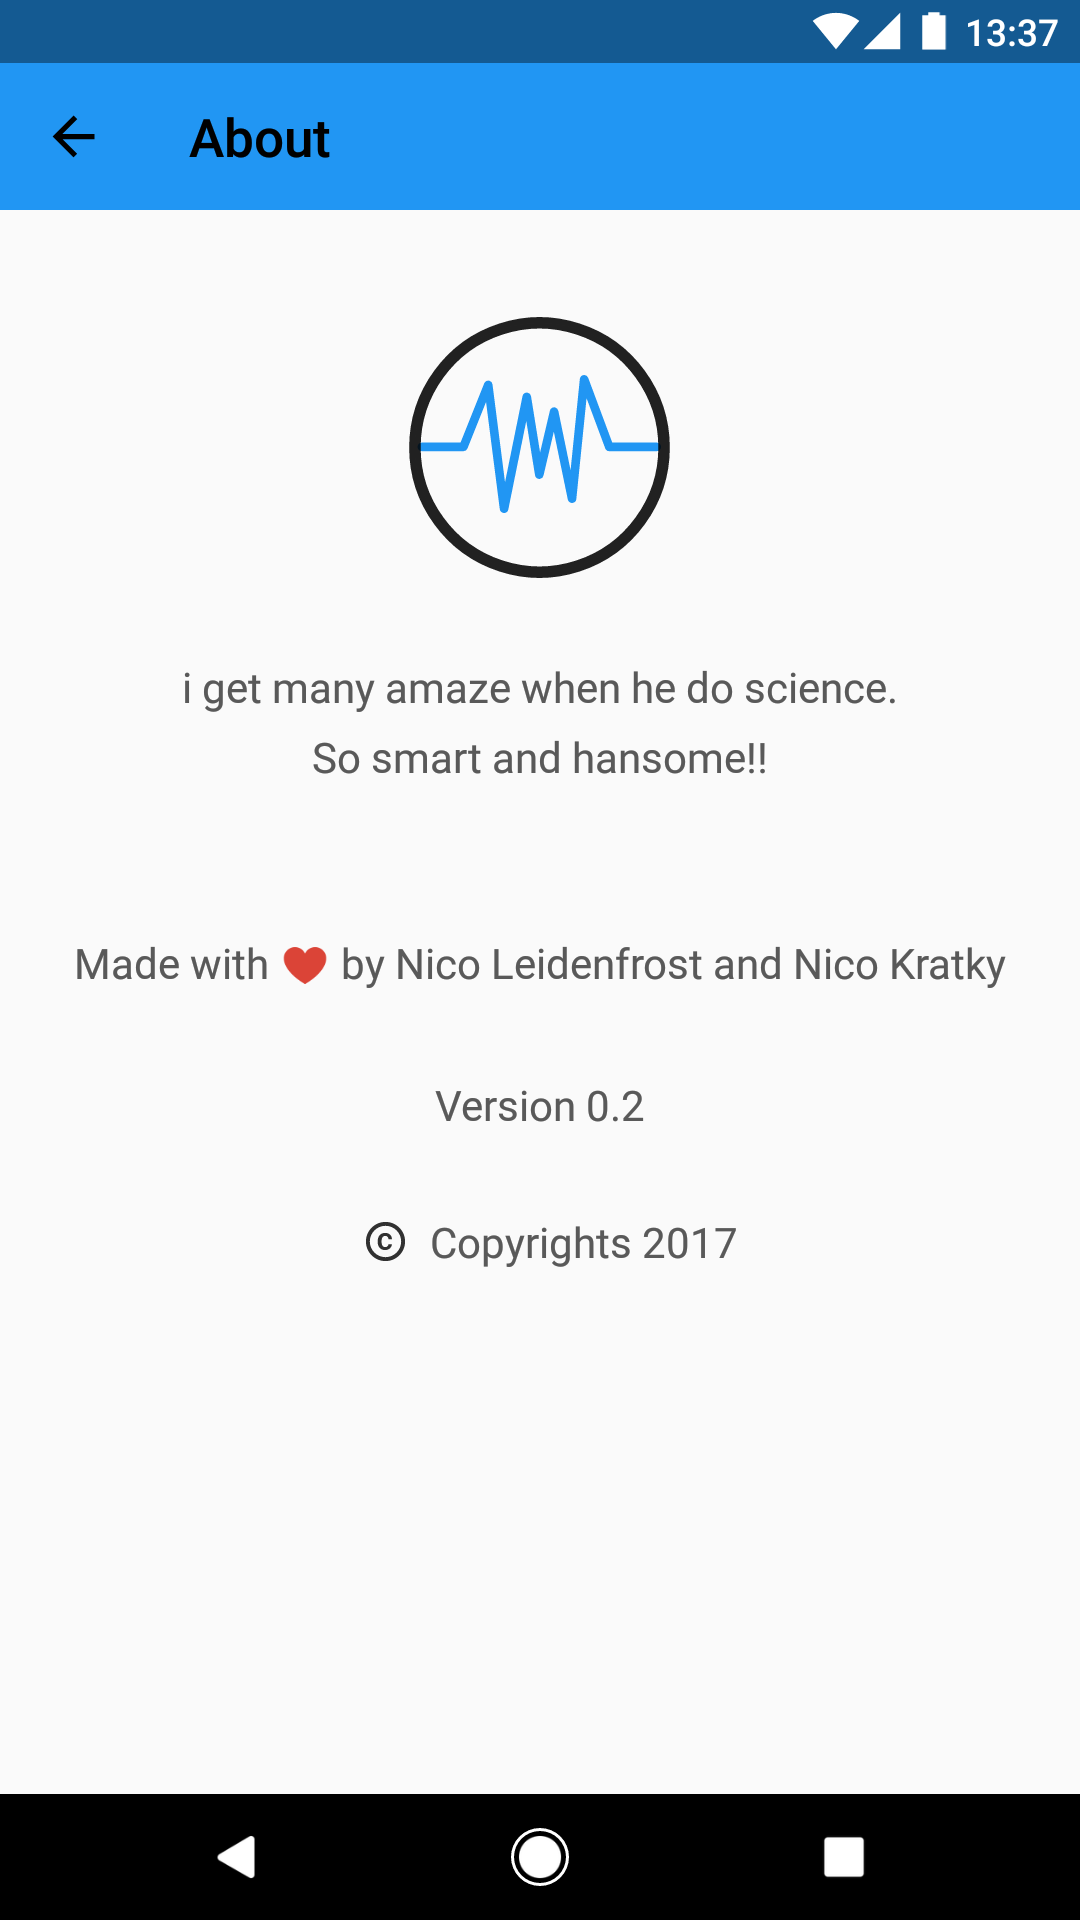
\includegraphics[height=7cm,keepaspectratio]{app_about}
	\end{tabular}
	\caption{Screenshots of App}
	\label{fig:appscreenshots}
\end{figure}

\section{Implementation}

\subsection{Libraries}
The Android client was implemented using a small number of libraries:
\begin{itemize}
	\item \textbf{Android SDK}

	The standard libraries included in the Android platform itself \cite{AndroidSDK}.

	\item \textbf{GramocAlgorithm-client}

	The Java implementation of the GSDEP client developed along with this project \cite{GramocAlgorithm-client}.

	\item \textbf{MPAndroidChart}

	An easy to use but also powerful open source 2 dimensional chart library for Android \cite{MPAndroidChart}.

	\item \textbf{android-about-page}

	This library allows to simply create an about page for your Android application \cite{android-about-page}.
\end{itemize}

\subsection{Components}
In order to build this Android application following components were used:

\begin{itemize}
	\item Activity
	\item Service
	\item NavigationDrawer
	\item Toolbar
	\item LineChart
	\item GramocAlgorithmClient
	\item Intent
	\item Thread
\end{itemize}

\subsection{Activity}
``An activity is a single, focused thing that the user can do.'' \cite{AndroidActivity} An activity is the main entry point of an application, it takes care of creating a new window and loading all the User Interface (UI) elements. Activities are usually shown as a full-screen window, but they can also be used as a floating window or even be embedded inside of another activity by implementing an ActivityGroup. Inside the Android-system, activities are managed as a stack, this means when a new activity is started it will be placed on top of this stack and become the running activity, the other activities are placed below this one in the stack and therefore remain inactive. The lifecycle of such an activity can be described as in Figure \ref{fig:activitylifecycle}.

\begin{figure}[H]
	\centering
	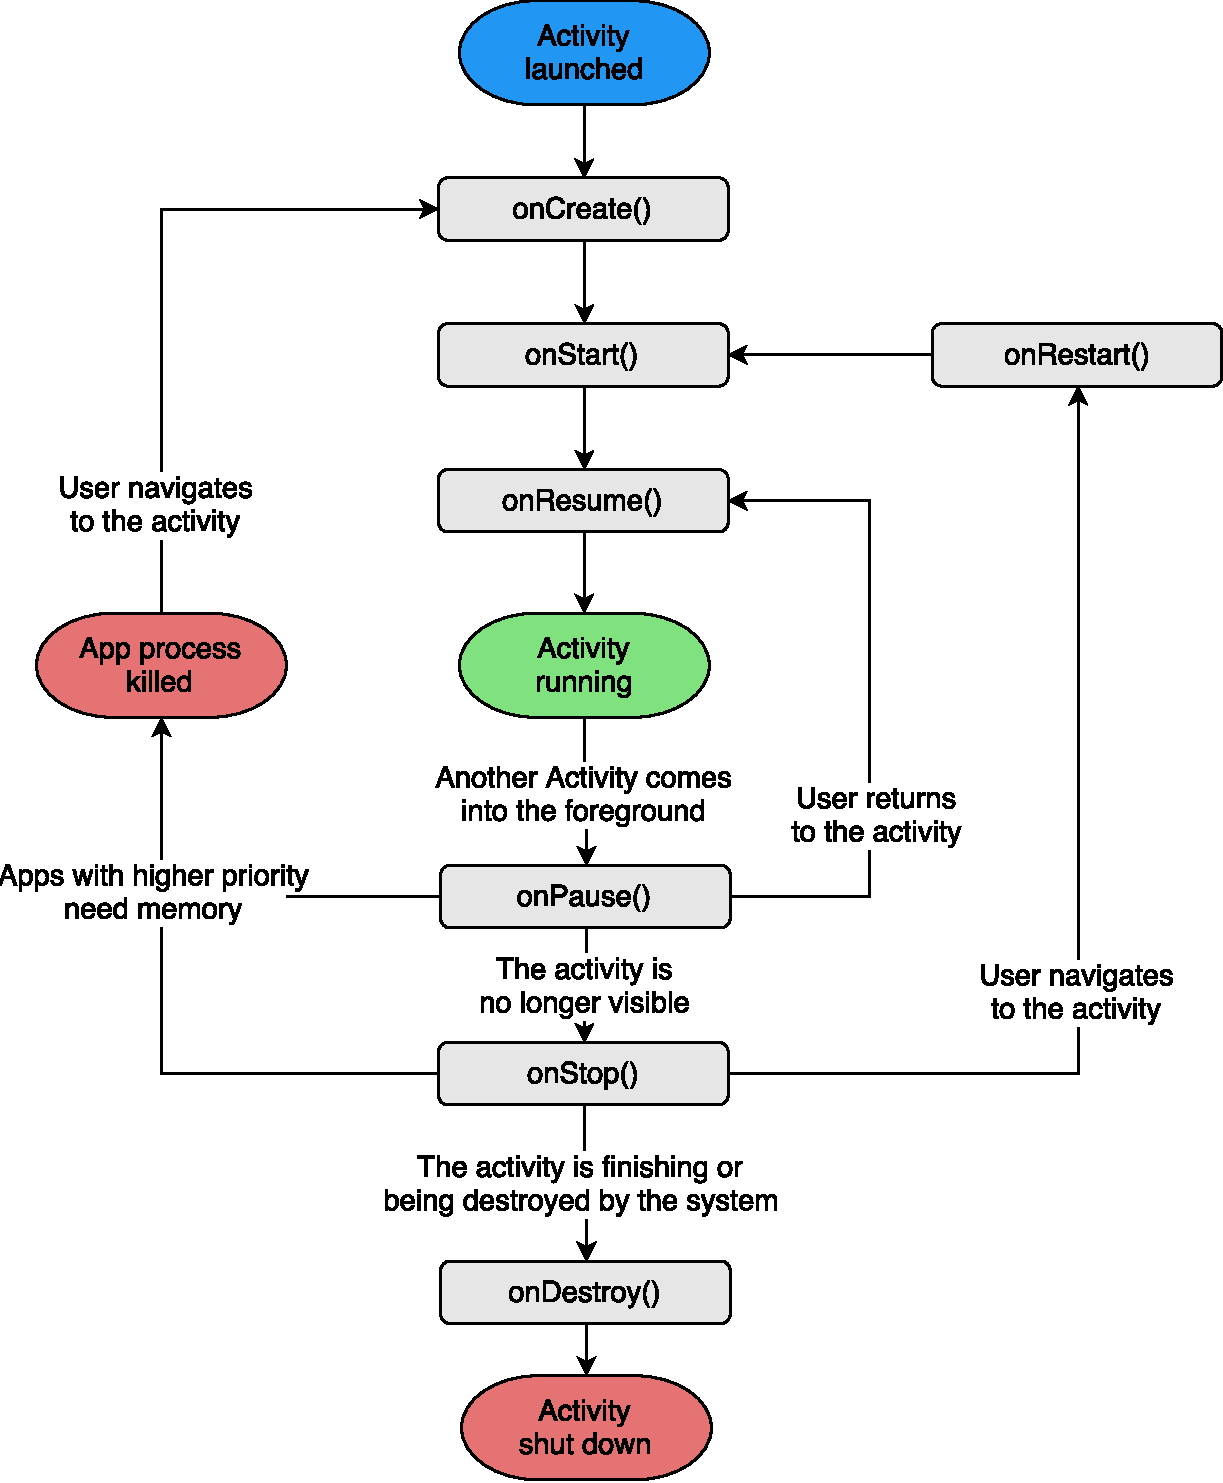
\includegraphics[width=10cm,keepaspectratio]{android-activity-lifecycle}
	\caption{Flowchart showing the lifecycle of an Android-activity}
	\label{fig:activitylifecycle}
\end{figure}

\subsection{Service}
A service is used to perform long-running operations in the background, because it's there it does not need a user interface like an activity. Once started a service can persist even if the user switches to another application. If another component binds itself to the service, it enables the possibility of interprocess communication (IPC). A typical example for a service is to handle network connections through it. The lifecycle is described as in Figure \ref{fig:servicelifecycle}.

\begin{figure}[H]
	\centering
	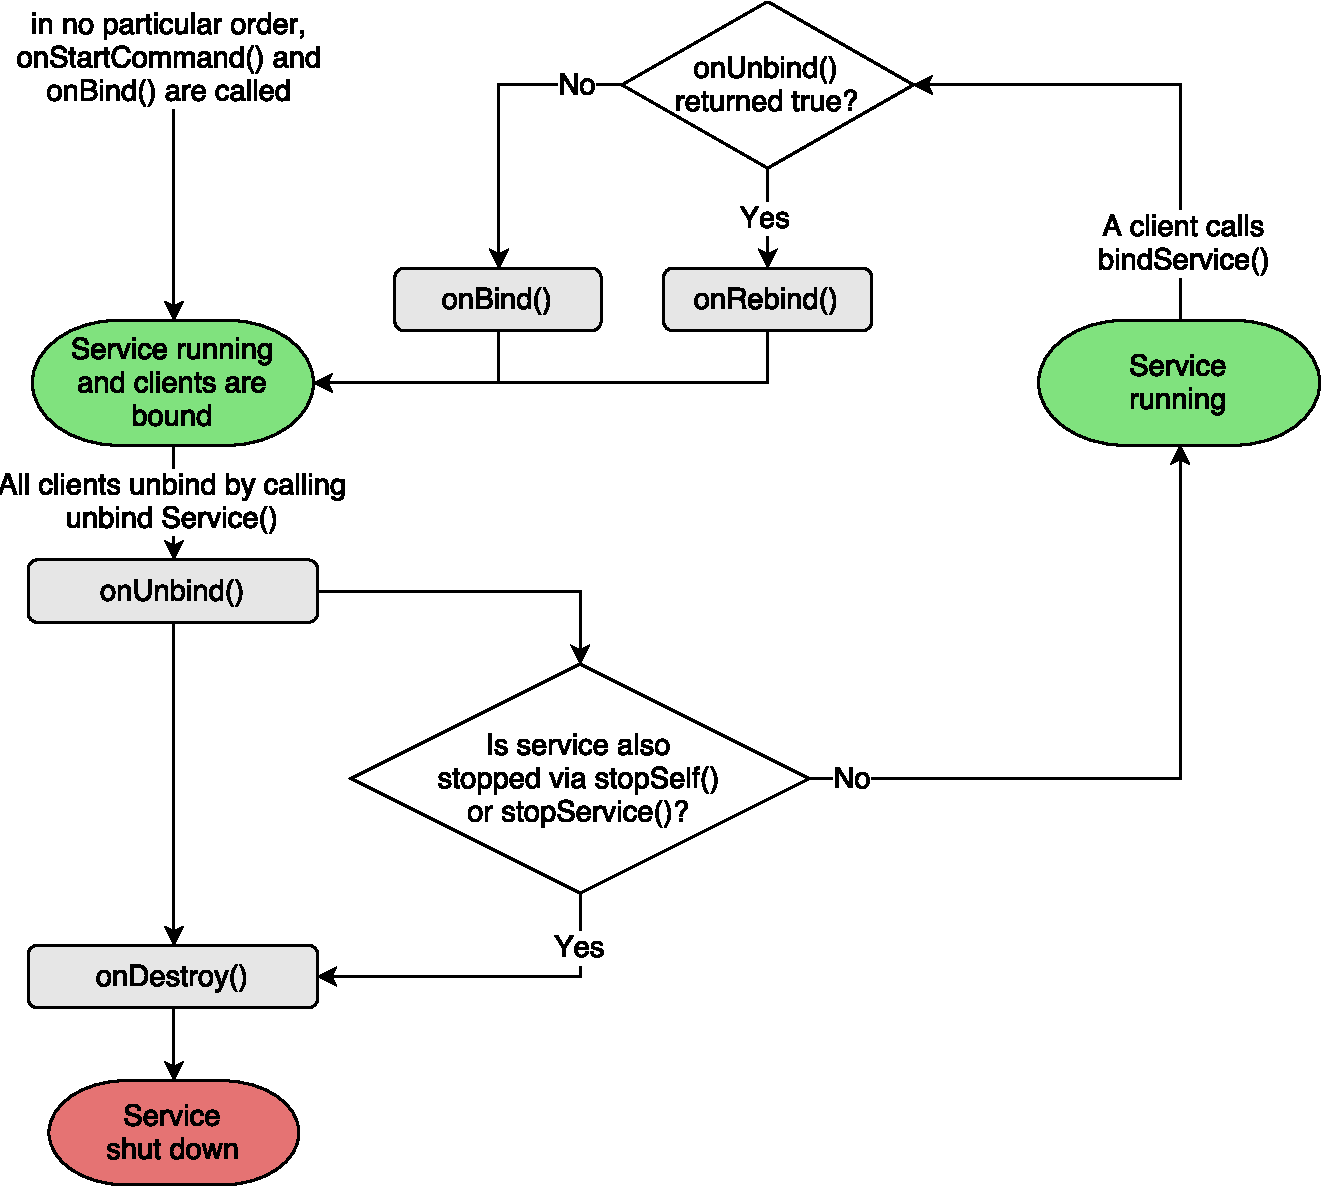
\includegraphics[width=10cm,keepaspectratio]{android-service-lifecycle}
	\caption{Flowchart showing the lifecycle of an Android-service}
	\label{fig:servicelifecycle}
\end{figure}

\subsection{NavigationDrawer}

\subsection{Toolbar}

\subsection{LineChart}

\subsection{GramocAlgorithmClient}

\subsection{Intent}

\subsection{Thread}

\subsection{Problems}


\part{Lessons Learned}
\part{Implementationphase 2}

%Literaturverzeichnis
\clearpage
\addcontentsline{toc}{chapter}{\bibname}

\bibliographystyle{bababbrv}
%options: babplain, babunsrt, bababbrv, babalpha
%         babplain-fl etc: first/lastname
%         babplain-lf etc: last/firstname
\bibliography{references}     %BibTeX-Datei literatur.bib


%%%----------------------------------------------------------

%%%Messbox zur Druckkontrolle
\chapter*{Messbox zur Druckkontrolle}



\begin{center}
{\Large --- Druckgröße kontrollieren! ---}

\bigskip

\Messbox{100}{50} % Angabe der Breite/Hoehe in mm

\bigskip

{\Large --- Diese Seite nach dem Druck entfernen! ---}

\end{center}



\end{document}
